
\chapter{Rešerše}
\label{reserse}

    V~této kapitole budou popsány podstatné pojmy pro pochopení práce, jako je uživatelská zkušenost, fyziologická data a~zařízení využívaná pro měření dat. Jednotlivé podkapitoly jsou vybrány na základě již existujících řešení zaobírajících se touto problematikou.

    \section{Ergonomie}
    Při návrhu produktů má z~pohledu psychologie zásadní roli ergonomie. Tento obor, též nazývaný lidský faktor, se zabývá studováním lidských schopností a~jeho chování na pracovišti za účelem vytvoření co nejlepšího produktu, aby bylo dosaženo ideálního používání lidmi~\cite{wiki:ergonomie}. 
    
    Hlavními přínosy jsou zvýšení bezpečnosti na pracovišti a~ochrana zdraví. Z~pohledu ekonomického je dosaženo vyšší efektivity práce a~tím zvýšení výdělku. 
    
    Svou roli hraje také v~oboru informačních technologií. Při návrhu nového softwaru je zásadní brát v~potaz lidský faktor především z~pohledu kybernetické bezpečnosti, kde jsou hackerské útoky cíleny také na psychologii člověka. Je tedy nutné vytvářet bezpečnostní opatření, jenž minimalizují škody způsobené těmito útoky. Poznatky ergonomie se hojně využívají i~při návrhu a~tvorbě uživatelských rozhraní, kde je za cíl maximalizovat pozitivní uživatelskou zkušenost.
    
    \section{Uživatelská zkušenost, interakce člověk-počítač}
    \label{user_experience}
    Uživatelská zkušenost (angl. User Experience, UX) je definovaná jako: \uv{Vnímání a~reakce člověka vyplývající z~použití nebo předpokládaného použití produktu, systému nebo služby.}~\cite{what_is_UX} 
    
    
    Pro analýzu a~zlepšení uživatelské zkušenosti vznikl obor nazývající se \textbf{UX design}. Pro dobrou uživatelskou zkušenost je důležité nejprve definovat potenciálního uživatele a~cíl produktu. Obecně lze důležité aspekty rozdělit následovně:
    \begin{itemize}
        \item užitečnost,
        \item použitelnost,
        \item zkušenost.
    \end{itemize}
    
    Podle potenciálního uživatele UX designéři určí, které aspekty jsou pro produkt více, či méně důležité a~tím určí nároky na výsledný produkt. V~oboru informační technologie lze jako produkt označit uživatelské rozhraní, jenž zprostředkovává interakci člověka a~počítače.
    
    \vspace{5mm}
    
     \textbf{Interakce člověk-počítač} (angl. Human-Computer Interaction, HCI) je druh komunikace, při níž dochází k~přenosu informací mezi člověkem a~počítačem, která spočívá v~interakci programátora, operátora či uživatele s~počítačem na základě přesně stanovených pravidel~\cite{hci}. 
    
    \begin{figure}[H]
        \centering
        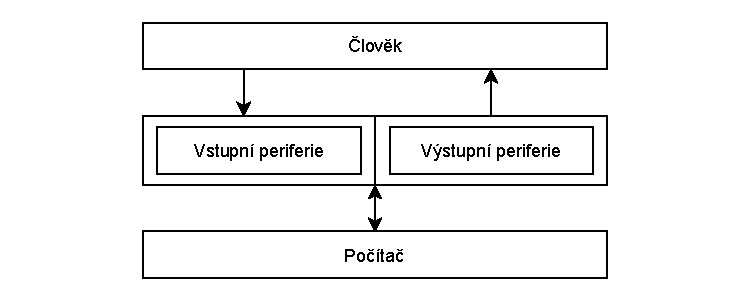
\includegraphics[width=\textwidth]{obrazky-figures/HCI.pdf}
        \caption{Schéma interakce člověk-počítač.  Vstupní informace jsou počítači předávány např. pomocí klávesnice, hlasového vstupu apod. Výstupní informace předává počítač člověku pomocí monitoru, tiskárny, hlasového výstupu apod.~\cite{hci}}
        \label{fig:hci}
    \end{figure}
    
    
    \section{Autonomní nervový systém}
    \label{nervous_system}
    
    Lidské tělo lze z~technického hlediska brát jako otevřený systém (obr.~\ref{fig:human_system}), jenž na základě signálů od smyslových orgánů (vstup) reaguje, vyhodnocuje situaci a~provádí odpovídající akce (výstup). Řízení celého systému má na starosti nervová soustava člověka, jenž je rozdělena na podsystémy. Pro kontrolu a~řízení fyziologických funkcí slouží autonomní nervový systém. 
    
    \begin{figure}[H]
        \centering
        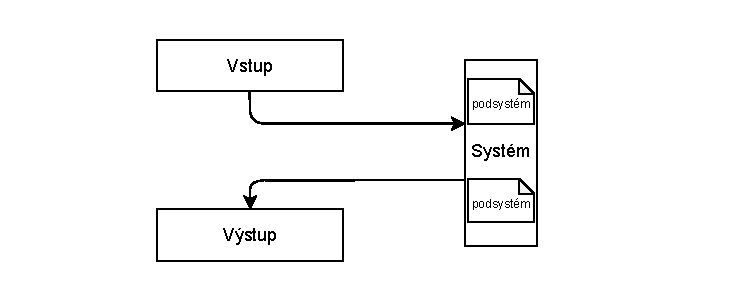
\includegraphics[width=\textwidth]{obrazky-figures/human_system.pdf}
        \caption{Schéma otevřeného systému.}
        \label{fig:human_system}
    \end{figure}
    
    Autonomní nervový systém (ANS), jehož centra jsou uložené podél páteře, je součást centrální nervové soustavy. Hlavní činností je regulace tělesné teploty, krevního tlaku, tepové frekvence, správná funkce útrobní svaloviny apod. Tyto funkce se obecně nazývají viscerální (útrobní) funkce~\cite{ans}.  
    
    \subsection{Anatomie autonomního nervového systému}
    Autonomní nervový systém se dělí na \textbf{sympatikus} a~\textbf{parasympatikus}. Tyto části jsou aktivovány na základě činnosti a~vnitřním stavu člověka~\cite{wiki_ans}.
    
    \textbf{Sympatikus} je aktivní v~situacích náročných na organismus (stres, boj o~život). Hlavní činností je uvolňování energie z~těla za účelem zvýšení výkonnosti člověka. Při jeho aktivaci lze pozorovat zvýšený srdeční tep, krevní tlak, zrychlený dech, rozšířené zornice apod. Jeho vliv na organismus je katabolický\footnote{Štěpení vysokomolekulárních prvků (bílkoviny, tuk) na jednoduché produkty za účelem vzniku energie.}~\cite{ans_s_p}.
    
    \textbf{Parasympatikus} se aktivuje v~klidových situacích (spánek, odpočinek, trávení jídla). Jeho činností je zpomalení funkcí těla a~výroba energie do zásoby. Při činnosti dochází ke zpomalení srdečního tepu, snížení krevního tlaku, zúžení zornic a~přesun krve do vnitřních orgánů~\cite{ans_s_p}.
    
    \begin{figure}[H]
        \centering
        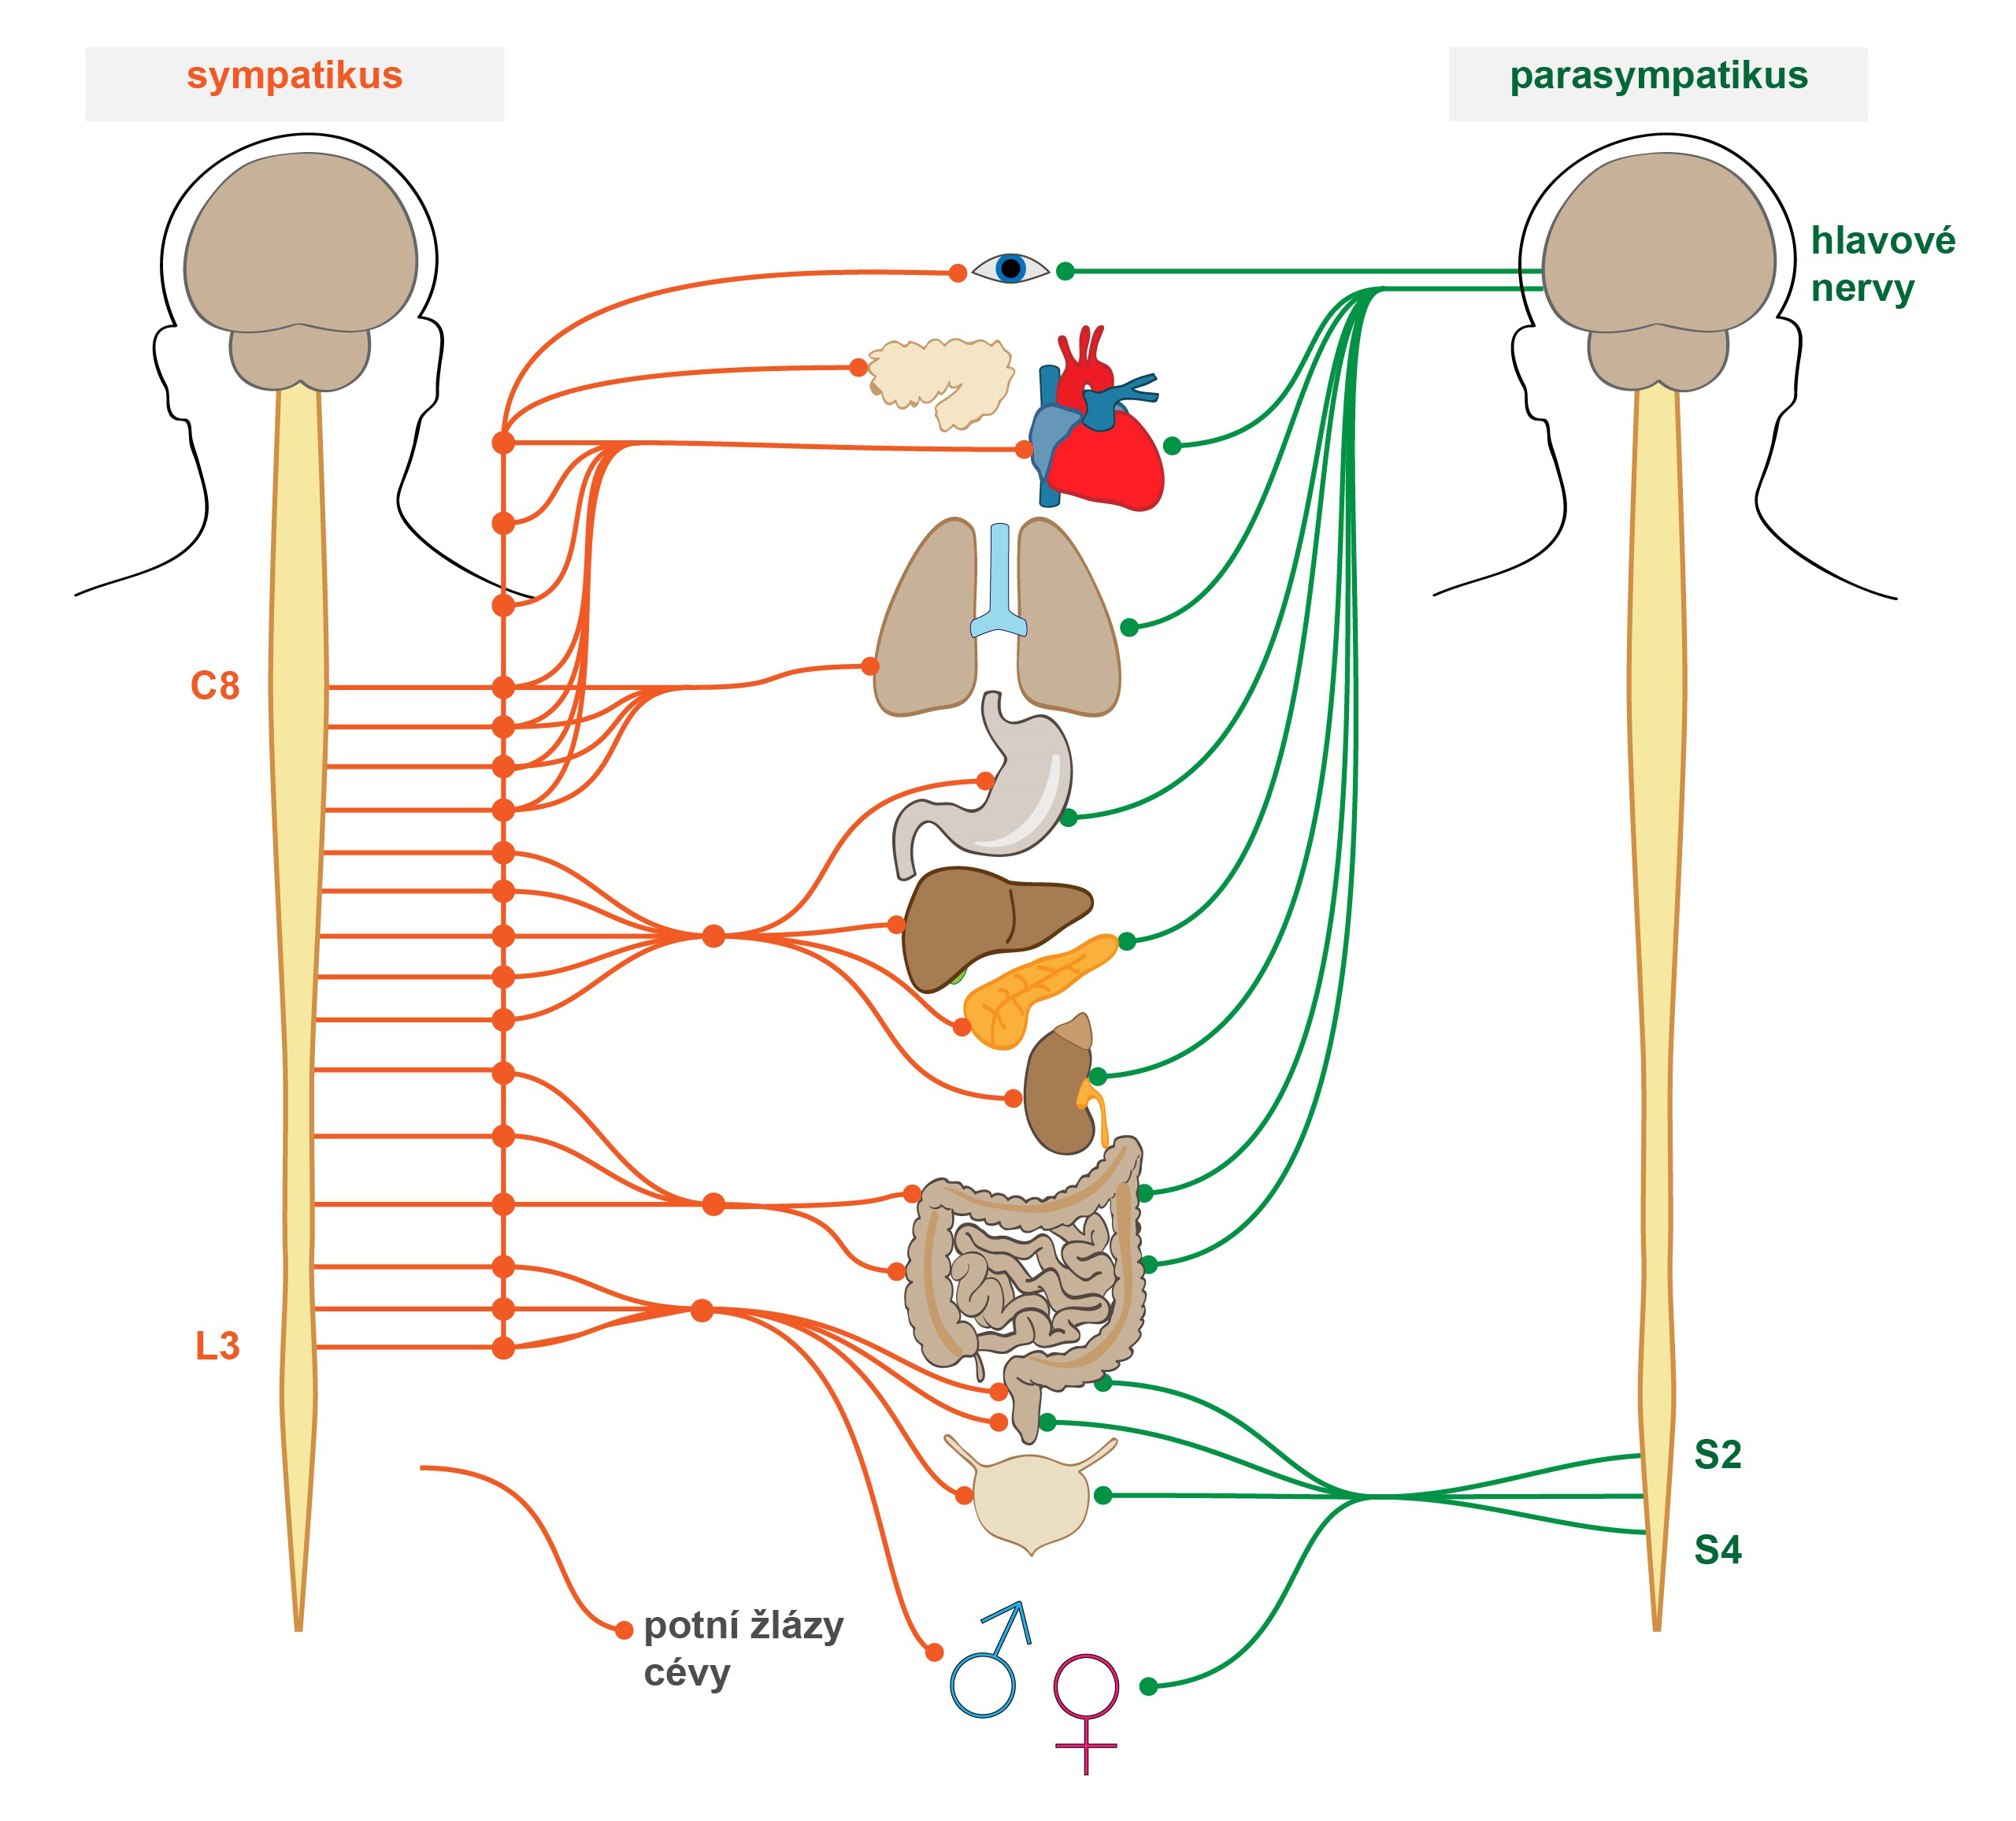
\includegraphics[scale=0.3]{obrazky-figures/sympatikus_parasympatikus.png}
        \caption{Anatomie autonomního nervového systému. Vlákna sympatiku jsou napojeny na míchu v~oblasti mezi prvním hrudním a~druhým bederním obratlem. Parasympatická vlákna jsou vyvedena z~mozku a~z~křížové části míchy. (Převzato z~\cite{ans})}
        \label{fig:symp_parasymp}
    \end{figure}
    
    \subsection{Stimulace autonomního nervového systému}
    Činnost ANS je automatická a~člověk si ji neuvědomuje. Aktivace ANS je možná na základě vnitřního stimulu (nemoc, jed v~těle), či pomocí vnějších podnětů (vysoké pracovní nároky, krizové situace). Pro stimulaci ANS v~rámci experimentů není možné, ani etické použít reálné stimuly, nicméně díky moderním technologiím a~empatii člověka lze tyto situace napodobit. Příkladem mohou být emoce vyvolané při sledování filmu, nebo hraní počítačové hry. Empatie člověka umožňuje vcítění do druhé osoby, nebo fiktivní (virtuální) postavy a~jeho situace. Pro skutečný prožitek a~vzbuzení odpovídajících emocí však pouhá empatie nestačí. Pro stimulaci nervové soustavy je důležitý především zážitek z~vlastní minulosti, fóbie jedince a~nebo instinkty člověka vytvořené evolucí a~vývojem. Dosud nejvěrnější simulaci reality umožňuje tzv. virtuální realita. Vnější podněty mohou být:
    \begin{itemize}
        \item vizuální,
        \item zvukové,
        \item čichové,
        \item hmatové,
        \item chuťové.
    \end{itemize}
    
    Z~nichž většinu vnímaných člověkem tvoří právě vizuální a~zvukové, čímž se stávají zásadními faktory mající vliv na emoční stav člověka. 
    
    \section{Emotivita člověka a~členění emocí}
    \label{emotivita}
    Emotivita člověka označuje celkovou citovou složku člověka, jejímž základem jsou emoce. Pojem emoce je definovaný jako: \uv{označení psychické funkce, která sestává ze tří komponent: citového zážitku, neuroendokrinních a~vegetativních (útrobních) procesů. Dimenze emocí: úroveň vzrušení, pocit příjemného či nepříjemného a~event. napětí a~uvolnění. Emoce byly pokládány za prožívání vzrušení, nebo vegetativních změn. Pocity příjemného a~nepříjemného signalizovaly biologickou hodnotu podnětu (pozitivní, negativní). Nověji jsou pokládány za integraci vzrušení a~kognitivního zpracování situace. Komplexnost emocí se vyvinula jako biologicky účelné spojení zážitků a fyziologických změn.}~\cite{vykladovy_slovnik}
    

    
    \begin{figure}[H]
        \centering
        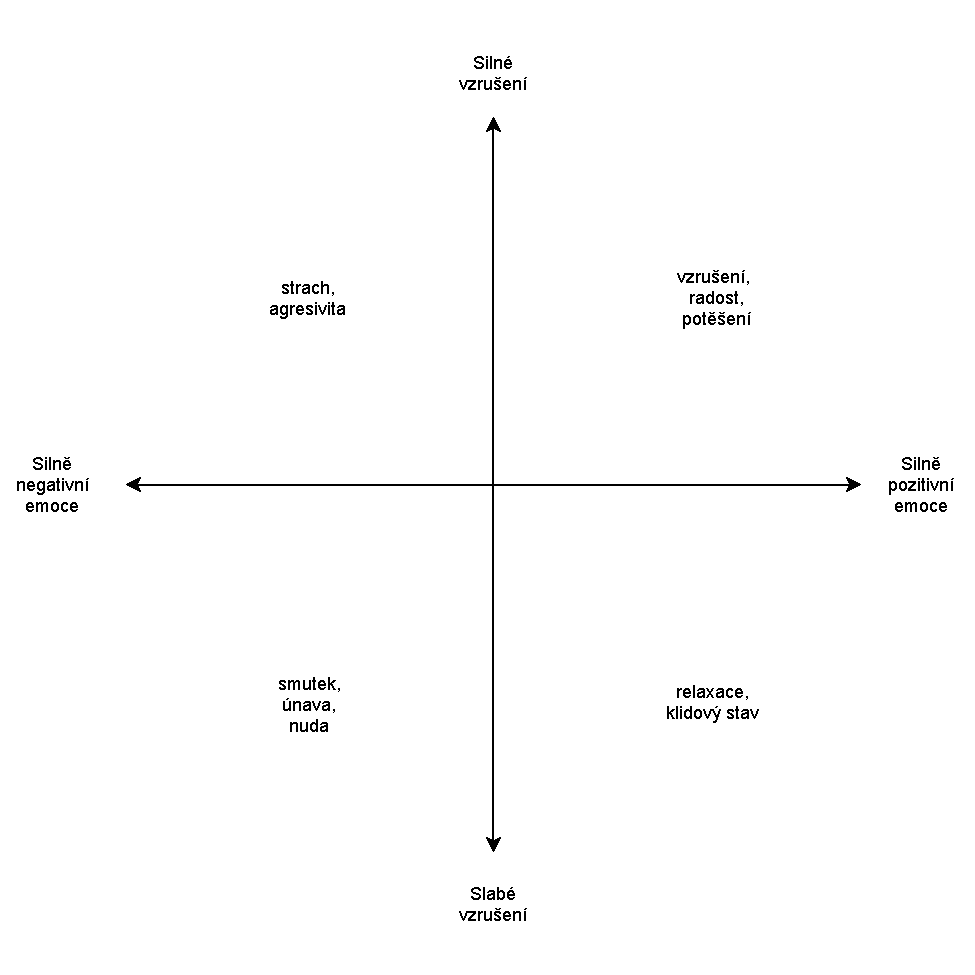
\includegraphics[scale=0.85]{obrazky-figures/emoce_graf.pdf}
        \caption{Graf členění emocí. Klasifikace na základě míry intenzity vzrušení a~pozitivity emoce.}
        \label{fig:emoce_graf}
    \end{figure}
    
    Emoce lze dělit na základní a~tzv. odvozené. Jako základní jsou obecně definovaný tyto:
    \begin{itemize}
        \item strach,
        \item smutek,
        \item hněv,
        \item radost,
        \item znechucení,
        \item překvapení.
    \end{itemize}
    
    Výhodou základních emocí je, že jsou snadno fyziologicky rozpoznatelné (výraz v~obličeji, zrychlený tep apod.). Nicméně pro psychologii takto generické členění není dostačující a~proto se v současné době, na základě výzkumů, rozlišuje až 27 odvozených emocí~\cite{Cowen201702247}.
    
   
    
    \section{Popis fyziologických dat a~jejich měření}
    \label{popis_dat_mereni}
        Při vytváření uživatelských rozhraní se využívá mnoho technik pro zajištění, co nejlepší uživatelské zkušenosti. Mezi nejčastější praktiky se řadí dotazníky, pozorování uživatele při práci, myšlení nahlas apod. \newline
        Současné studie se zabývají tím, jak analyzovat uživatelskou zkušenost na základě fyziologie člověka. Cílem fyziologie je pochopení a~vysvětlení fyzikálních, biochemických a~biologických principů fungovaní procesů v~lidském těle~\cite{wiki:fyzio}.
        
        \subsection{Srdeční pulz}
        \label{srdecni_tep}
        Srdeční pulz, neboli tep člověka, lze považovat za jeden ze základních signálů v~lidském těle. Pulz je tlaková vlna vyvolaná vypuzením krve z~levé komory do aorty~\cite{wiki:fyzio_sledovani}. Při jeho měření lze pozorovat tyto vlastnosti:
        \begin{itemize}
            \item frekvenci,
            \item pravidelnost,
            \item kvalitu.
        \end{itemize}
        
        Měření probíhá pomocí elektrod připevněných na kůži, či optickými snímači.
        
        Při měření \textbf{elektrodami} se jedná o~Elektrokardiografii (EKG)\footnote{\url{https://www.wikiskripta.eu/w/Elektrokardiografie}}. Výhodou oproti optickým snímačům je přímé snímání elektrické aktivity srdce. Touto metodou lze získat frekvenci i~pravidelnost srdečního tepu. Metoda je hojně využívána pro lékařské účely, neboť je velmi přesná a~poskytuje podrobné údaje. Detailní pohled na EKG signál zobrazuje obrázek~\ref{fig:ecg}.
        
        \begin{figure}[H]
            \centering
            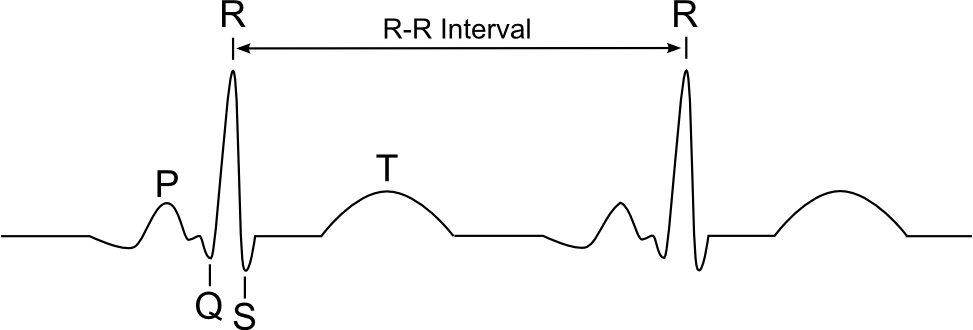
\includegraphics[width=\textwidth]{obrazky-figures/Ecg.png}
            \caption{Měřitelné artefakty v~EKG. Hlavním prvkem je R-R interval, určující frekvenci srdečního tepu. P~vlna značí depolarizaci předsíní srdce. Komplex vln QRS signalizuje depolarizaci komor. Vlna T~charakterizuje následnou repolarizaci komor.~\cite{wiki_ecg} Zdroj: Wikimedia Commons~\cite{wiki:commons}}
            \label{fig:ecg}
        \end{figure}
        
        \textbf{EKG přístroj} neboli elektrokardiograf je zdravotnický přístroj, jenž citlivě snímá elektrickou aktivitu srdce v~čase. Pomocí elektrod, které se připojují na různé části těla, snímá elektrické změny na srdci a~zaznamenává je jako tzv. EKG křivku. Díky měření na více místech zároveň lze přesněji analyzovat srdeční činnost. 
        
        \begin{figure}[H]
            \centering
            
\includegraphics[width=\textwidth]{obrazky-figures/ekg_dev.png}
            \caption{Elektrokardiograf a ukázka EKG křivky zaznamenávané na speciální papír. (Převzato z~\cite{web_ekg})}
            \label{fig:ekd_dev}
        \end{figure}
        
        Pro běžné užití existují tzv. hrudní pásy. Hlavní výhodou je bezdrátový přenos dat do mobilního telefonu, nebo sporttesteru umožňující volný pohyb při snímání a~měření srdeční aktivity.
        
        \begin{figure}[H]
            \centering
            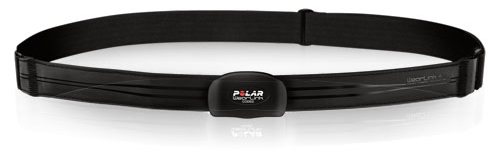
\includegraphics{obrazky-figures/Hrudni-pas.png}
            \caption{Běžný hrudní pás pro měření životních funkcí. (Převzato z~\cite{wiki:commons})}
            \label{fig:hrudni_pas}
        \end{figure}
        
        Metoda využívající \textbf{optické snímače} se nazývá Fotopletysmografie (angl. Photoplethysmography, PPG)\footnote{\url{https://en.wikipedia.org/wiki/Photoplethysmogram}}. Pro snímání vyžaduje dvě optoelektronické součástky. LED diodu jako zdroj světelného paprsku a~ fotodiodu, nebo fotorezistor jako detektor odraženého světla. Vysílaný světelný paprsek proniká lidskou tkání a~částečně se absorbuje. Detektor odraženého světla následně měří množství zbytkového světla (viz obrázek~\ref{fig:ppg_scheme}). 
        
        \begin{figure}[H]
            \centering
            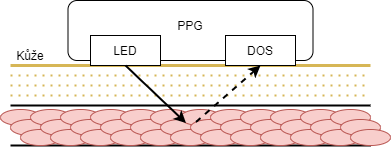
\includegraphics[width=\textwidth]{obrazky-figures/ppg_scheme.png}
            \caption{Princip měření srdečního tepu pomocí PPG. LED dioda jako zdroj světla prosvicuje kůži a~odražené světlo zachycuje detektor odraženého světla (DOS), typicky fotodioda.}
            \label{fig:ppg_scheme}
        \end{figure}

        Změna objemu krve procházející měřeným místem je přímo úměrná změně intenzity záření. Při měření touto metodou je nutné počítat se slábnutím signálu podle vzdálenosti měřícího zařízení od srdce a~podle toho patřičně zesílit získaný signál. PPG signál je zobrazen a~popsán na obrázku~\ref{fig:ppg_fig}.
        
        \begin{figure}[H]
            \centering
            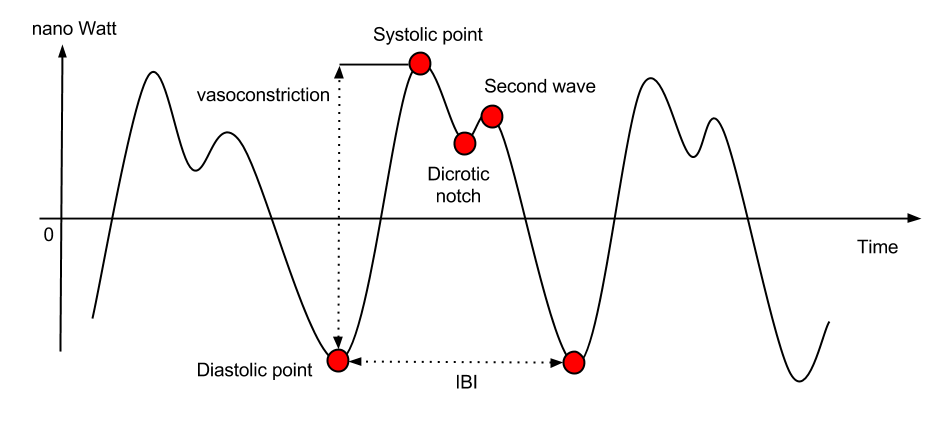
\includegraphics[width=\textwidth]{obrazky-figures/ppg.png}
            \caption{Artefakty pozorovatelné v~PPG signálu. Diastolické body (diastolic points) označují lokální minima PPG signálu využívaná pro výpočet IBI (čas mezi dvěma tlakovými vlnami). Pomocí IBI je možné vypočítat frekvenci srdečního tepu. Systolické body (systolic points) značí lokální maxima signálu. Dikrotický zářez (Dicrotic notch), za předpokladu, že se subjekt nehýbe, lze využít pro detekci srdečních onemocnění. Zdroj: Empatica Support~\cite{empatica_support}}
            \label{fig:ppg_fig}
        \end{figure}
        
         Nevýhodou Fotopletysmografie je zpoždění měření a~zanesení chyby způsobené zesílením signálu v~závislosti na vzdálenosti měření od srdce. Kvalitu dat ovlivňuje i~nedostatečně přiložený senzor k~tělu, nebo barva kůže. Mezi výhody patří snadné využití technologie v~nositelné elektronice a~tudíž pohodlné a~nerušivé využití uživateli.
     
        
        \subsection{Galvanická odezva kůže}
        \label{gsr}
        Galvanická odezva kůže, nebo také elektrodermální aktivita (EDA) je vlastnost lidského těla, která způsobuje neustálé změny elektrických charakteristik pokožky~\cite{eda}. Při fyzické zátěži nebo při prožívání emocí mozek vysílá signál do pokožky, za účelem zvýšení pocení. I když není dotekem možné pocítit zvýšenou potivost, tak se elektrické vlastnosti pokožky mohou změnit. Měřené veličiny se dělí na:
        \begin{itemize}
            \item endosomatické,
            \item exosomatické.
        \end{itemize}

        Endosomatické veličiny jsou takové, které jsou měřeny bez vnějšího zdroje napětí. Mezi tyto veličiny patří například potenciál kůže, tedy rozdíl napětí mezi dvěma místy na těle. 
        
        Exosomatické veličiny se měří za pomocí vnějšího elektrického zdroje. Elektrické zdroje mohou být stejnosměrné i~střídavé. Zařízení se stejnosměrným zdrojem napětí jsou využívány častěji, neboť střídavé zdroje vyžadují sofistikovanější zařízení a~jsou nákladnější na výrobu. Jako exosomatické veličiny se označují kožní vodivost nebo kožní odpor~\cite{eda_book}. Při analýze signálu lze pozorovat dvě složky:
        \begin{itemize}
            \item úroveň tónické vodivosti pokožky
            \item fázovou reakci vodivosti kůže
        \end{itemize}  
        
        \begin{figure}[H]
            \centering
            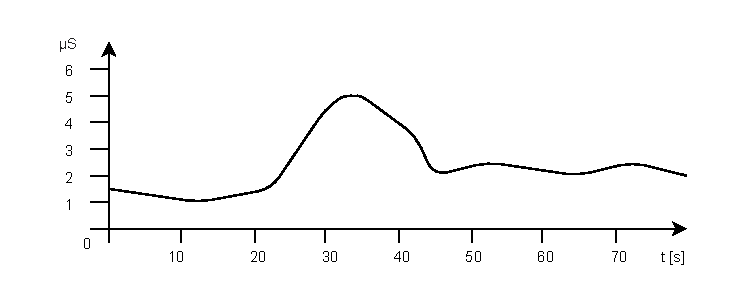
\includegraphics[width=\textwidth]{obrazky-figures/Gsr.pdf}
            \caption{Signál elektrodermální aktivity s~výraznou fázovou reakcí způsobenou podnětem.}
            \label{fig:gsr_signal}
        \end{figure}
 
        \textbf{Fázová reakce vodivosti kůže} je spjata s~krátkými událostmi, jenž mohou vyvolat zvuky, pachy, apod. Fázové změny se v~signálu projevují jako náhlé \uv{špičky}. Fázová vodivost se označuje také jako odezva vodivosti kůže (angl. Skin Conductance Response, SCR).
        
        \begin{figure}[H]
            \centering
            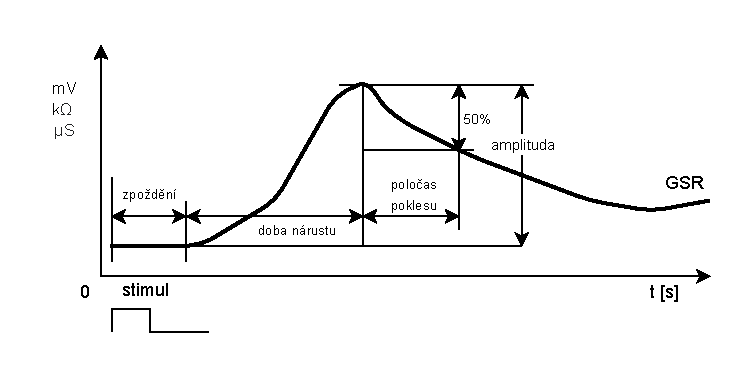
\includegraphics[width=\textwidth]{obrazky-figures/gsr_scr.pdf}
            \caption{Detailní pohled na fázovou reakci vodivosti kůže na vnější stimulaci. Po krátkém zpoždění začíná tzv. doba nárustu a~následně dochází k~zotavení (tzv. poločas poklesu).}
            \label{fig:scr_graph}
        \end{figure}
        
        \textbf{Tónická vodivost kůže} (angl. Skin Conductance Level, SCL) je artefakt signálu, který je možné pozorovat v~delším časovém intervalu měření, typicky v~řádech desítek sekund až desítek minut. Pro získání tónické vodivosti kůže je nutné vyfiltrovat fázické špičky a~následně se hodnota SCL vypočítá jako aritmetický průměr v~rámci zvoleného časového okna. 
        
        
       
        \subsection{Oční reakce}
        \label{eye_tracking}
        Monitorování pohybu očí (angl. eye tracking) je metoda využívaná pro měření oční aktivity. Pomáhá určit jak oči reagují na podněty, nebo které objekty uživatelé pozorují, případně v~jakém pořadí uživatel objekty sleduje.
        
        Z~očí je také možné vyčíst jak se uživatel cítí. Obecně je možné pozorovat na očích únavu, případně stres. Monitorování očí probíhá pomocí kamer a~algoritmů, které se zaměřují pouze na oblast očí a~jejich pohyb. Při pozorování očních zornic lze sledovat:
        \begin{itemize}
            \item pohyb očí,
            \item mrkání,
            \item kontrakci zornic.
        \end{itemize}
        
        Pozorování může ovlivnit faktor okolního prostředí. Především okolní osvětlení a~sluneční záření, kdy při zvýšené intenzitě okolního světla dochází k~zúžení zornic, naopak v~tmavém prostředí dochází k~rozšíření zornic. Proto je nutné, pro validitu experimentu, vytvořit pracovní prostředí se stabilními světelnými podmínkami.
        
        \begin{figure}[H]
            \centering
            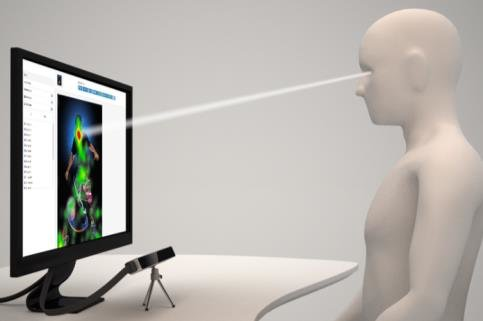
\includegraphics[width=\textwidth]{obrazky-figures/Eye-tracking-setup.png}
            \caption{Pracovní prostředí pro monitorování pohybu očí. (Převzato z~~\cite{eye_tracking_setup})}
            \label{fig:eye_tracking_setup}
        \end{figure}
        
        Monitorování pohybu očí lze využít v~mnoha oblastech. Od léčení mentálních poruch až po zlepšení každodenního života lidí. Časté uplatnění nalézá pro navrhování a~úpravu uživatelského rozhraní, neboť poskytuje velmi přesná data o~tom, co je pro uživatele zajímavé a~pomáhá zvolit design i~uspořádání objektů. Dále se využívá v~automobilovém průmyslu, kde pomáhá sledovat bdělost a~pozornost řidičů, a~tím zvyšuje bezpečnost silničního provozu.
        
        \subsection{Mozková aktivita}
        Mozková aktivita se často zaznamenává pomocí diagnostické metody zvané Elektroencefalografie (EEG). Jelikož metoda využívá povrchové elektrody, řadí se mezi neinvazivní. Aktivita mozku se projevuje změnou polarizace neuronů, tím dochází k~elektrickým změnám, které jsou snímány elektrodami.
            
        Pro správné měření je důležité rovnoměrně rozmístit povrchové elektrody pomocí předem daného schématu, jehož příklad je na obrázku~\ref{fig:eeg_scheme}, kde počet elektrod odpovídá počtu sledovaných kanálů. Elektrody lze rozmístit jednotlivě, nebo existují standardizované elektrodové čepice pro snadnější použití. Nevýhodou měření elektrodami je omezená délka experimentu, neboť pro dobrý kontakt je nutné použít vodivý gel, který postupně vysychá a~ztrácí své vlastnosti. Dále musí být zajištěno klidné prostředí a~minimalizovat veškerý pohyb pozorovaného.
        
        \begin{figure}[H]
            \centering
            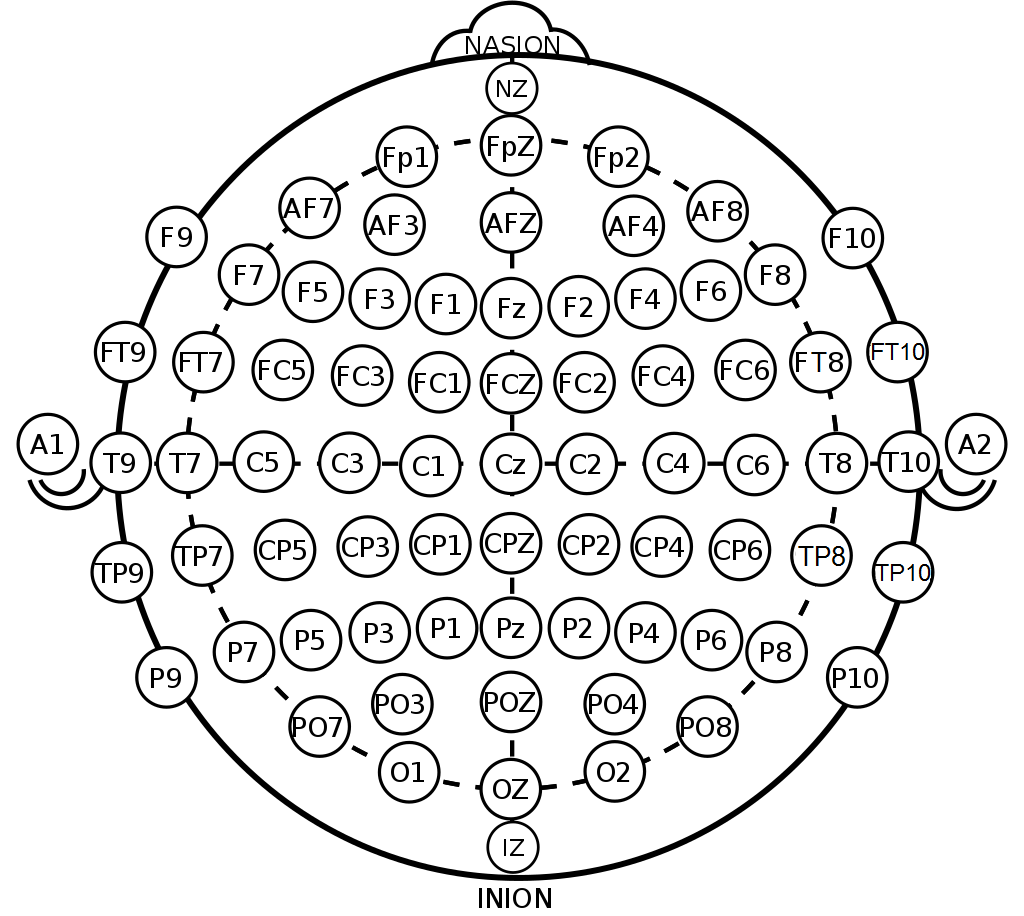
\includegraphics[width=\textwidth]{obrazky-figures/eeg_scheme.png}
            \caption{Příklad schématu rozmístění elektrod podle standardu. Jednotlivé elektrody jsou označeny písmeny(A = Ušní lalůček; C = Centrální; P = Temenní (Parental); F = Čelní (Frontal); O = Týlní kost (Occipital); T = Temporální) a~čísly (lichá čísla pro elektrody umístěné nad levou mozkovou hemisférou, sudá čísla pro elektrody nad pravou hemisférou).~\cite{wiki_eeg} }
            \label{fig:eeg_scheme}
        \end{figure}
            
        EEG nalézá využití v~neurologii a~psychiatrii. Pomáhá monitorovat a~diagnostikovat choroby jako jsou migrény, epilepsie nebo kóma. Snímání mozkových aktivit mozku pomáhá postiženým pacientům ovládat různá zařízení a~přístroje (tzv. neurofeedback)~\cite{wiki_eeg}.
        
         \subsection{Krevní tlak} 
        Krevní tlak je tlak, kterým působí krev na stěny cév. Krevní tlak se dělí na: 
        \begin{itemize}
            \item arteriální,
            \item systolický,
            \item diastolický.
        \end{itemize}
            
        Při měření se nejčastěji zjišťuje arteriální tlak. Jeho hodnotu může ovlivnit věk, stres, aktivita apod. Nízký tlak (pod 100/60 mmHg) se označuje jako hypotenze, naopak vysoká hodnota (nad 140/90 mmHg) jako hypertenze. Obvyklý tlak dospělého jedince je 120/80 mmHg. 
        
        Měřit krevní tlak lze na horních i~dolních končetinách pomocí arteriální kanyly nebo tonometru, kde pro validní hodnoty je nutné zvolit správnou velikost manžety~\cite{wiki:fyzio_sledovani}. 
            
        \subsection{Teplota} 
        Teplota člověka vyjadřuje poměr mezi vytvořeným teplem v~organismu a~odvedeným teplem z~těla. Na teplotu má vliv věk, denní doba, hormony, zdravotní stav, tělesná aktivita a~okolní prostředí. Běžná teplota je v~rozmezí 36.0\,-\,36.9\,$^\circ$C. Vyšší teplota se označuje jako horečka, naopak nižší hodnota jako podchlazení. Smrtelné hodnoty jsou pod 34\,$^\circ$C a~nad 42\,$^\circ$C. Měření probíhá pomocí teploměru~\cite{wiki:fyzio_sledovani}.
            
        \subsection{Dech} 
        Dýchání je základní činnost člověka zajišťující přívod kyslíku do organismu. Jako jediná fyziologická funkce je ovlivnitelná vlastní vůlí. Dýchání ovlivňuje aktivita člověka, prostředí, onemocnění, věk i~stres. Při měření se zjišťuje:
        \begin{itemize}
            \item pravidelnost,
            \item kvalita,
            \item rychlost.
        \end{itemize}
        
        
        Dechová frekvence se dělí na: eupnoe (normální frekvence), tachypnoe (zvýšená frekvence), bradypnoe (snížená frekvence), apnoe (bezdeší)~\cite{wiki:fyzio_sledovani}.
        
        \section{Vliv emotivity člověka na fyziologické funkce}
        \label{emotion_to_physio}
        Fyziologická data jsou možnost jak sledovat emoční stav člověka v~každodenním životě lidí. Důkazem tvrzení jsou provedené studie, v~nichž bylo využito různých postupů ke vzbuzení emocí a~měření jejich vlivu na fyziologické funkce člověka.
        
        \vspace{3mm}
        
        Typickým příkladem jsou studie zabývající se měřením stresu různými postupy. Jednou z~nich je studie~\cite{detection_stress} zabývající se detekcí stresu pomocí krátkých ECG a~HRV signálů. Pro stimulaci byl použit tzv. \uv{stroop color word test}\footnote{SCWT: \url{https://www.ncbi.nlm.nih.gov/pmc/articles/PMC5388755/}}. Pro zpracování a~klasifikaci bylo využito více metod (FFT\footnote{FFT: Fast Fourier transform}, PNN\footnote{PNN: probabilistic neural network}, kNN\footnote{kNN: k--nearest neighbors algorithm}, binární klasifikace). Délka dat pro analýzu byla nejméně 25 sekund. Průměrná klasifikační úspěšnost byla mezi 91.66\% a~94.66\%. 
        
        Dále se studie zaměřují také na konkrétní emoce. Postupy ke vzbuzení emocí byly různé. Například byly použity audio podněty a~jako metriky byly zvoleny ECG s~EDA~\cite{audio_stimuli}. Další kategorií jsou vizuální podněty. Ty mohou být pouze jako obrázky, nebo videonahrávky. 
        
        V~případě použití obrázků jako stimulů jsou obrázky obvykle získávány z~různých databází, např. Geneva affective picture database (GAPED). Studie~\cite{wearable_emotion_gaped} využívala tuto databázi a~měřila EDA i~srdeční tep. Srdeční tep byl získáván PPG senzory. Podněty byly zobrazeny vždy 6~sekund a~následně bylo 15 sekund pro volbu emoce metodou SAM~\cite{herbon2006emotions}. Ke klasifikaci bylo využito SVM\footnote{Support Vector Machines} i~kNN. Klasifikace probíhala do 4~skupin podle míry vzrušení a~pozitivity emoce (viz~\ref{emotivita}). Úspěšnost klasifikačních metod a~postupů se pohybovala v~rozmezí od 65\,\% do 87\,\%. 
        
        Druhou variantou jsou videonahrávky použité jako podněty. Ukázkou je studie~\cite{video_emotion} měřící 4~fyziologické funkce (EEG, EDA, sledování dechu, ECG) najednou. Snaha byla získat data pro 6~emocí +~klidový stav. Podněty byly zobrazovány po dobu 10 sekund a~poté vždy následovala 30 sekund dlouhá relaxační fáze. Ke klasifikaci bylo využito více metod jako SVM, kNN nebo LSTM\footnote{Long Short--Term Memory}. Výsledky metod byly následně porovnávány. Nejlepších výsledků dosahovala metoda LSTM a~její modifikace A--LSTM\footnote{Attention--Long Short--Term Memory}. Z~měřených metrik vykazovala nejlepší výsledky EEG. 
        
        Kromě obvyklých postupů bylo také zkoumáno, jaký mají vliv počítačové hry na emoční stav člověka~\cite{fps_emotions}. Studie porovnávala zpětnou vazbu hráčů s~naměřenými daty EDA a~PPG senzory. Ukázalo se, že existuje silná korelace mezi zpětnou vazbou a~fyziologickými daty, jenž byly naměřeny. Další studie~\cite{vr_emotions}, porovnávala rozdíl mezi podněty přijímanými pomocí VR Headsetu a~běžné 2D obrazovky. Jako metriky byly zvoleny: srdeční tep, galvanická odezva kůže. Měření se zúčastnilo 33~dobrovolníku a~probíhalo pomocí dvou zařízení. Srdeční tep byl měřen běžným chytrým náramkem a~galvanická odezva kůže za pomocí PIP Biosenzoru\footnote{\url{https://thepip.com/en-eu/}}. Po zpracování výsledků se použití VR Headsetu projevilo pouze v~galvanické odezvě kůže. Je možné, že malé změny v~hodnotách srdečního tepu způsobilo také zvolené zařízení.
        
        \vspace{3mm}
        
        